\documentclass[12pt,a4paper]{article}

\usepackage{viu-mrob-memoria}

\setviutitle{Coordinación distribuida local de múltiples AGV para el transporte cooperativo de cargas heterogéneas en entornos industriales}
\setviustudent{Jorge Luis Mayorga Taborda}
\setviututor{Jose Ignacio Iñiguez Amigot}
\setviuedition{2025--26}
\setviudate{20 de mayo de 2026}

\begin{document}

\makeviuwordcover

\pagenumbering{roman}
\begin{viuabstract}
Este Trabajo Fin de Máster plantea el estudio de la coordinación distribuida local de múltiples AGV para el transporte cooperativo de cargas heterogéneas en entornos industriales. El problema se ubica en bodegas automatizadas donde una sola unidad móvil puede resultar insuficiente para desplazar cargas voluminosas, pesadas o con propiedades inerciales variables, y donde el uso de un control centralizado puede limitar la escalabilidad y la robustez del sistema. El objetivo del trabajo es diseñar, implementar y evaluar una arquitectura de control cooperativo distribuido, basada en consenso y con compensación adaptativa o robusta, que permita coordinar varios AGV a partir de información local. La metodología propuesta combina revisión bibliográfica, modelado planar del sistema robot-carga, definición de grafos de comunicación, diseño de una estrategia nominal y una estrategia adaptativa, simulación cuantitativa en Python y validación aplicada en CoppeliaSim. La comparación se realizará mediante métricas de error de seguimiento, error de formación, esfuerzo de control, tiempo de convergencia y robustez cooperativa frente a variaciones de masa, desplazamientos del centro de masas, degradación de comunicación y perturbaciones externas. Como resultado esperado, se busca obtener una evaluación técnica reproducible que permita identificar las condiciones bajo las cuales el control cooperativo adaptativo mejora el desempeño frente a una estrategia nominal.

\keywords{control distribuido; cooperación multiagente; AGV; transporte cooperativo; CoppeliaSim.}
\end{viuabstract}

\frontindexes
\pagenumbering{arabic}

\section{Introducción}

La automatización de bodegas y centros de distribución ha incrementado el uso de vehículos guiados automáticamente y robots móviles para tareas de transporte interno. En sistemas de alta rotación, estos robots permiten reducir desplazamientos manuales, mejorar la repetibilidad de las operaciones y conectar estaciones de almacenamiento, preparación y despacho. Sin embargo, una parte importante de las soluciones industriales se diseña bajo una hipótesis operativa sencilla: cada robot transporta una unidad de carga compatible con sus dimensiones, capacidad mecánica y modo de sujeción. Esta hipótesis funciona bien cuando los objetos son homogéneos, pero resulta menos flexible cuando aparecen cargas heterogéneas, voluminosas, frágiles o demasiado pesadas para un único AGV.

El transporte cooperativo multi-robot aborda precisamente ese tipo de situaciones. En lugar de asignar una carga a un único vehículo, varios agentes móviles actúan de forma coordinada para desplazar un mismo objeto o para mantener una formación que permita soportar y guiar la carga. Desde el punto de vista de la robótica avanzada, el problema no consiste únicamente en desplazar robots en el plano, sino en diseñar reglas de interacción que permitan que un comportamiento colectivo emerja a partir de decisiones locales. Esta idea conecta directamente con los sistemas multiagente, la teoría de grafos, el control distribuido y los algoritmos de consenso.

El problema se vuelve más exigente cuando la carga transportada no se conoce con exactitud. En una bodega real, una misma plataforma puede manipular objetos con distintas masas, geometrías o distribuciones de peso. La incertidumbre en masa, inercia o centro de masas modifica la respuesta dinámica del sistema y puede degradar tanto el seguimiento de trayectoria como el mantenimiento de la formación entre AGV. Si además se impone una comunicación local, cada agente dispone solo de información parcial de sus vecinos y no de una visión completa del sistema. Este escenario motiva el uso de control cooperativo distribuido frente a soluciones centralizadas.

\subsection{Contexto industrial y problema de investigación}

En entornos industriales, los AGV y AMR suelen integrarse en flujos de producción, almacenamiento o intralogística. Las soluciones comerciales de gran escala demuestran que la coordinación de flotas puede ser altamente eficiente cuando las tareas son repetitivas y las cargas están normalizadas. No obstante, la cooperación física sobre una misma carga plantea una dificultad distinta: varios robots deben mantener relaciones geométricas, distribuir esfuerzos y responder a perturbaciones de forma coherente. En esta situación, el problema técnico principal no es solo la navegación individual, sino la coordinación dinámica del conjunto.

El problema de investigación de este TFM se formula así: cómo diseñar una estrategia de control cooperativo distribuido que permita a varios AGV transportar cargas heterogéneas bajo comunicación local y parámetros inerciales inciertos. La formulación se centra en el plano, con robots móviles de tracción diferencial o comportamiento cinemático equivalente, y con una carga rígida cuya masa o distribución inercial puede variar entre escenarios. La decisión de trabajar en el plano acota el problema y permite concentrar el esfuerzo en el diseño de control y cooperación.

\subsection{Soluciones actuales, límites y brecha de investigación}

Las soluciones existentes pueden agruparse en tres familias. La primera corresponde a esquemas centralizados, donde una unidad de planificación o control calcula las acciones del conjunto. Estos enfoques simplifican la coordinación global, pero pueden crear dependencia de un nodo central, aumentar los requisitos de comunicación y reducir la tolerancia a fallos. La segunda familia corresponde a arquitecturas líder-seguidor, en las que un robot o una referencia virtual organiza el movimiento de los demás. Esta solución reduce parte de la complejidad, aunque mantiene dependencia de un rol privilegiado y puede ser sensible a la pérdida o degradación del líder. La tercera familia corresponde a control distribuido y consenso, donde cada agente actualiza su acción a partir de información local y del estado relativo de sus vecinos.

La literatura de consenso y cooperación multiagente muestra que es posible coordinar vehículos sin requerir comunicación global, siempre que la topología de comunicación satisfaga condiciones mínimas de conectividad \cite{olfati2007consensus,ren2008distributed}. Sin embargo, en transporte cooperativo de cargas heterogéneas aparecen límites adicionales: la carga introduce acoplamiento físico entre agentes, los parámetros inerciales pueden ser inciertos y la degradación de la comunicación puede afectar directamente la formación. Por tanto, la brecha que aborda este TFM no es demostrar que el consenso existe, sino evaluar cómo una arquitectura cooperativa distribuida se comporta cuando el transporte de carga introduce incertidumbre dinámica y escenarios de operación más cercanos a una bodega industrial.

En el contexto industrial, las plataformas de bodega automatizada han demostrado que la coordinación de grandes flotas es viable cuando las unidades de carga, las estanterías y los flujos de trabajo están estandarizados. No obstante, esa madurez no resuelve completamente el caso de cargas heterogéneas que requieren cooperación física simultánea. En el primer caso, cada robot ejecuta una tarea individual dentro de una flota coordinada; en el segundo, varios robots deben actuar como un sistema mecánico distribuido. Esta diferencia justifica que el TFM se centre en cooperación y control, y no únicamente en planificación logística o gestión de flotas.

Desde el punto de vista académico, el trabajo se apoya en un conjunto de antecedentes consolidados: la teoría de consenso para sistemas multiagente, la coordinación de redes robóticas, la cooperación en sistemas de robots móviles y el transporte cooperativo de objetos \cite{bullo2009distributed,cao1997cooperative,dudek1996taxonomy,parker2008multiple}. Sin embargo, el interés del TFM está en articular esos elementos en un marco aplicado a AGV industriales con comunicación local y carga incierta. Por tanto, el aporte no se define como la invención de un principio de control completamente nuevo, sino como la formulación, implementación y evaluación rigurosa de una arquitectura cooperativa bajo condiciones de operación delimitadas.

\begin{table}[htbp]
\centering
\caption{Relación entre problema, brecha y respuesta metodológica.}
\begin{tabularx}{\textwidth}{>{\bfseries}p{0.30\textwidth}Y}
\toprule
Elemento & Planteamiento en el TFM \\
\midrule
Problema técnico & Transporte cooperativo de cargas heterogéneas con múltiples AGV bajo incertidumbre inercial. \\
Soluciones actuales & Control centralizado, líder-seguidor, consenso distribuido y enfoques de cooperación multi-robot. \\
Límites detectados & Dependencia de comunicación global, sensibilidad a parámetros de carga y evaluación limitada ante degradación del grafo. \\
Respuesta propuesta & Arquitectura de control cooperativo distribuido con comparación nominal/adaptativa en Python y CoppeliaSim. \\
\bottomrule
\end{tabularx}
\end{table}

\subsection{Plataforma propuesta y delimitación inicial}

El trabajo plantea dos niveles de plataforma. El primer nivel es una simulación cuantitativa en Python, donde se implementan el modelo, los controladores, las perturbaciones, las métricas y la generación de resultados. Este nivel será la base científica del trabajo porque permite controlar condiciones iniciales, repetir escenarios y comparar de forma justa estrategias de control. El segundo nivel es CoppeliaSim, usado como entorno de validación aplicada para representar la escena multi-AGV en una bodega, visualizar la cooperación y comprobar que el enfoque no queda reducido a una simulación abstracta sin conexión robótica.

La delimitación del TFM excluye la construcción física de AGV, la percepción real, la planificación global de rutas, la navegación SLAM y la certificación de seguridad industrial. Estas decisiones no reducen el valor del trabajo, sino que permiten focalizarlo en el núcleo académico: control y cooperación. La validación se realizará mediante escenarios simulados, con especial atención al seguimiento de trayectoria, mantenimiento de formación, esfuerzo de control, tiempo de convergencia y robustez frente a incertidumbre.

\begin{figure}[htbp]
\centering
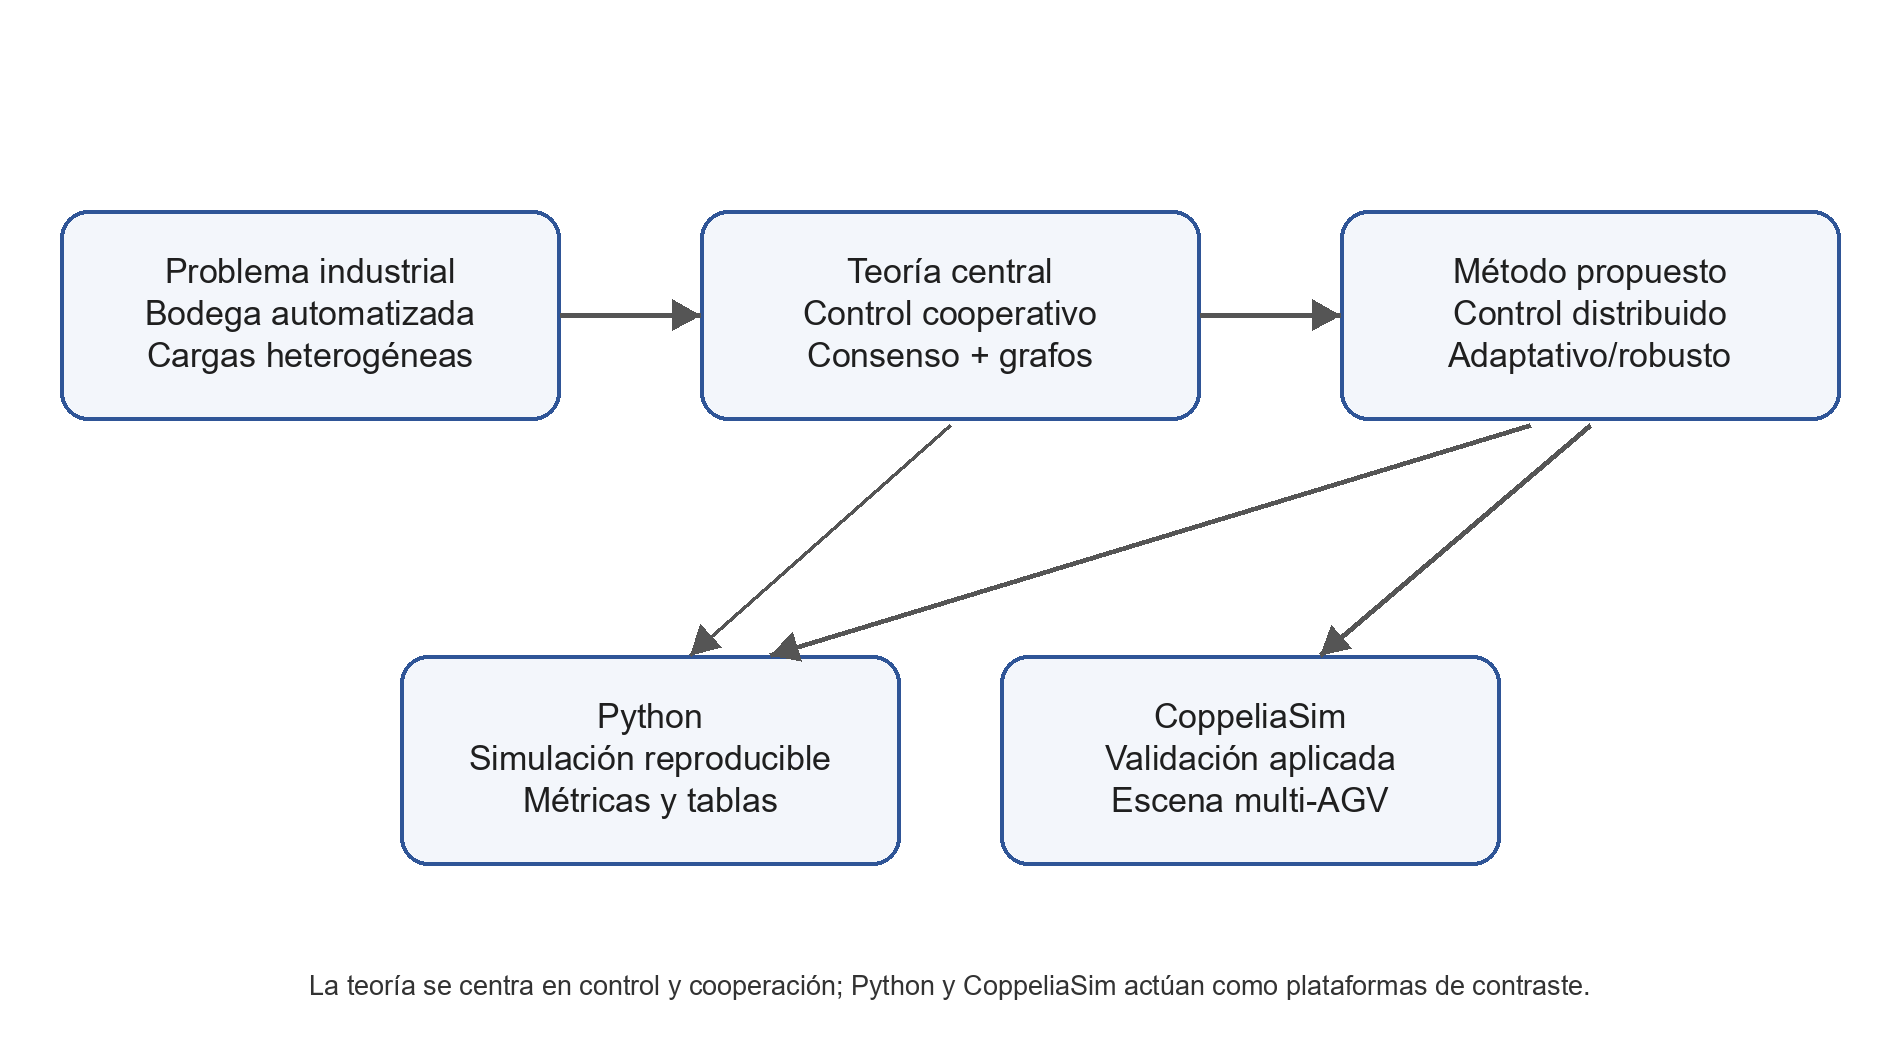
\includegraphics[width=0.92\textwidth]{assets/image3.png}
\caption{Arquitectura metodológica del TFM.}
\end{figure}

\subsection{Pregunta de investigación y justificación académica}

La pregunta de investigación que orienta el trabajo es la siguiente: ¿puede una arquitectura de control cooperativo distribuido, basada en consenso y con compensación adaptativa o robusta, mejorar el transporte de cargas heterogéneas por múltiples AGV bajo incertidumbre inercial y comunicación local, en comparación con una estrategia nominal? Esta pregunta es adecuada para un TFM de robótica y automatización porque integra modelado, control, cooperación, simulación y validación aplicada.

La justificación académica se apoya en tres argumentos. Primero, el problema pertenece al ámbito de la robótica móvil industrial y de los sistemas multiagente, áreas directamente vinculadas con el Máster Universitario en Robótica y Automatización de Procesos. Segundo, el trabajo exige aplicar conocimientos de control avanzado, modelado de sistemas y simulación robótica. Tercero, la evaluación comparativa permite producir evidencia cuantitativa, no solo una demostración visual. Con ello, el documento puede cumplir el doble carácter esperado: memoria técnica y estudio teórico-técnico.

La memoria se organizará de forma progresiva. En primer lugar, se delimita el problema y se ubican las soluciones actuales. En segundo lugar, se definen objetivos, hipótesis y alcance. En tercer lugar, se desarrolla la metodología de modelado, control, simulación y comparación. En la versión final se incorporarán el marco teórico completo, los resultados, el análisis, la validación y las conclusiones.

\section{Objetivos}

Los objetivos se formulan para que el trabajo sea evaluable mediante resultados técnicos. El objetivo general expresa el propósito principal, mientras que los objetivos específicos organizan el desarrollo en tareas verificables: modelado, cooperación, control, simulación, validación y comparación.

\subsection{Objetivo general}

Diseñar, implementar y evaluar una arquitectura de control cooperativo distribuido para múltiples AGV, basada en consenso y con compensación adaptativa o robusta, orientada al transporte de cargas heterogéneas bajo incertidumbre inercial en entornos industriales simulados.

\subsection{Objetivos específicos}

\begin{enumerate}
  \item Caracterizar el problema de transporte cooperativo de cargas heterogéneas en una bodega automatizada.
  \item Formular un modelo planar del sistema multi-AGV-carga con variables cinemáticas y dinámicas relevantes.
  \item Definir la cooperación entre AGV mediante grafos de comunicación local y condiciones de conectividad.
  \item Diseñar una estrategia nominal de control distribuido basada en consenso.
  \item Proponer una variante adaptativa o robusta frente a incertidumbre de masa, inercia o centro de masas de la carga.
  \item Implementar una plataforma de simulación reproducible en Python para comparar estrategias de control.
  \item Validar visualmente el comportamiento cooperativo en CoppeliaSim mediante una escena de bodega industrial.
  \item Evaluar las estrategias mediante métricas de seguimiento, formación, esfuerzo de control, convergencia y robustez cooperativa.
  \item Analizar los resultados para determinar en qué condiciones la cooperación adaptativa mejora o no a la estrategia nominal.
\end{enumerate}

\subsection{Alcance del TFM}

El alcance se define para mantener un equilibrio entre profundidad teórica y viabilidad técnica. El trabajo se concentrará en el control cooperativo distribuido para transporte de cargas en el plano. La plataforma experimental será simulada, pero la simulación se diseñará con criterios de reproducibilidad y trazabilidad de resultados.

El TFM incluye los siguientes elementos:
\begin{itemize}
  \item modelo planar de un sistema compuesto por múltiples AGV y una carga heterogénea;
  \item grafos de comunicación local para representar cooperación entre agentes;
  \item controlador nominal distribuido basado en consenso;
  \item controlador adaptativo o robusto frente a incertidumbre inercial;
  \item escenarios de variación de masa, desplazamiento del centro de masas, degradación de comunicación y perturbaciones;
  \item simulación cuantitativa en Python y validación aplicada en CoppeliaSim.
\end{itemize}

El TFM excluye explícitamente los siguientes elementos:
\begin{itemize}
  \item construcción o ensayo con AGV físicos reales;
  \item percepción visual, SLAM o navegación autónoma completa;
  \item planificación global de rutas en bodega;
  \item identificación experimental completa de parámetros inerciales;
  \item certificación de seguridad industrial o integración con sistemas productivos reales.
\end{itemize}

\section{Hipótesis de partida}

La hipótesis de partida orienta el diseño experimental y define una afirmación contrastable. En este TFM no se asume que la estrategia adaptativa será superior en todos los casos; se plantea que puede mejorar la consistencia del comportamiento cooperativo bajo determinadas formas de incertidumbre, con posibles costes en esfuerzo de control.

Hipótesis principal: una estrategia de control cooperativo distribuido basada en consenso y con compensación adaptativa o robusta puede reducir la degradación del desempeño del transporte multi-AGV frente a incertidumbre inercial de la carga, en comparación con una estrategia nominal, siempre que el grafo de comunicación mantenga conectividad suficiente.

Hipótesis secundarias: primero, la estrategia adaptativa reducirá el error de seguimiento y el error de formación en escenarios con variación de masa o desplazamiento del centro de masas. Segundo, la mejora de robustez puede implicar un incremento moderado del esfuerzo de control. Tercero, la ventaja del enfoque cooperativo disminuirá cuando la comunicación local se degrade de forma severa. Cuarto, una métrica de robustez cooperativa permitirá resumir la degradación relativa del desempeño entre controladores y escenarios.

\section{Metodología}

La metodología se diseña como una investigación aplicada, cuantitativa y experimental en simulación. El propósito es comparar estrategias de control bajo condiciones controladas, manteniendo la misma plataforma, las mismas trayectorias y las mismas perturbaciones para cada controlador. La metodología también incorpora una validación aplicada en CoppeliaSim, cuyo objetivo es visualizar y comprobar la coherencia robótica del comportamiento cooperativo.

La lógica metodológica sigue la secuencia planteada para el TFM completo: definir el problema, analizar cómo se resuelve actualmente, identificar límites, proponer una plataforma, formular un método de control cooperativo, compararlo en Python, validarlo en CoppeliaSim y discutir los resultados. En la presente entrega se desarrolla hasta el diseño metodológico; los resultados y conclusiones se incorporarán en fases posteriores.

\subsection{Diseño de investigación}

El diseño de investigación es comparativo porque enfrenta una línea base nominal con una estrategia adaptativa o robusta. Es cuantitativo porque el desempeño se evaluará mediante métricas numéricas, y es experimental en simulación porque las variables independientes se modificarán de manera controlada. La comparación se realizará sobre escenarios equivalentes para evitar que las diferencias observadas provengan de condiciones iniciales, trayectorias o parámetros no controlados.

La unidad de análisis será el sistema cooperativo completo, no un AGV individual. Esto implica que el desempeño se medirá sobre la carga, la formación y el conjunto de acciones de control. La decisión es coherente con la teoría central del trabajo: el objetivo no es optimizar un robot aislado, sino evaluar cómo la cooperación local permite resolver una tarea que supera la capacidad o conveniencia de un único agente.

La investigación no tendrá como variable principal la calidad gráfica de la simulación, sino el comportamiento del sistema de control. Por ese motivo, las métricas se calculan sobre estados, errores y acciones de control. CoppeliaSim se incorporará como herramienta para comprobar la coherencia de la escena robótica y para comunicar de forma visual el transporte cooperativo, pero la comparación formal se basará en registros numéricos.

\subsection{Fases del trabajo}

El desarrollo se organizará en fases incrementales. Cada fase produce un artefacto verificable que alimenta la siguiente, evitando que la memoria dependa de resultados no reproducibles o de decisiones no documentadas.

\begin{enumerate}
  \item Revisión bibliográfica sobre consenso, control distribuido, cooperación multi-robot y transporte cooperativo.
  \item Definición del sistema robot-carga, supuestos de modelado y variables de estado.
  \item Diseño de grafos de comunicación local para representar la cooperación entre AGV.
  \item Implementación del controlador nominal basado en consenso.
  \item Diseño e implementación del controlador adaptativo o robusto.
  \item Configuración de experimentos reproducibles en Python.
  \item Construcción de una escena de validación en CoppeliaSim.
  \item Ejecución de escenarios, generación de métricas y producción de figuras.
  \item Análisis comparativo, discusión de limitaciones y redacción de conclusiones.
\end{enumerate}

\subsection{Plataforma de simulación y validación}

Python será la plataforma principal de simulación. En esta capa se implementarán el modelo, los controladores, las perturbaciones y las métricas. La elección responde a la necesidad de reproducibilidad: los experimentos podrán ejecutarse desde archivos de configuración, registrar resultados brutos y generar tablas o figuras sin intervención manual. CoppeliaSim se usará como plataforma de validación aplicada. Su función será representar el entorno de bodega, los AGV, la carga y el movimiento cooperativo, conectando el análisis de control con una escena robótica interpretable.

La comunicación entre ambos niveles se planteará de forma pragmática. Python funcionará como banco de pruebas cuantitativo; CoppeliaSim reproducirá uno o varios escenarios representativos para mostrar el comportamiento cooperativo. Esta separación evita que las limitaciones gráficas o de configuración de CoppeliaSim condicionen la comparación científica, y al mismo tiempo evita que el TFM quede desconectado de una aplicación robótica visible.

En el repositorio del TFM, cada experimento se documentará mediante archivos de configuración y salidas separadas en resultados brutos, resultados procesados, tablas y figuras. Esta organización permite repetir ejecuciones, revisar parámetros y asociar cada figura de la memoria con un experimento concreto. La trazabilidad es especialmente importante porque la evaluación final no debe depender de capturas aisladas, sino de una cadena reproducible desde configuración hasta resultado.

\subsection{Método propuesto}

El método nuevo se plantea como una arquitectura de control cooperativo distribuido. Cada AGV calcula su acción a partir de su estado local, el error respecto a la tarea cooperativa y la información recibida de sus vecinos en el grafo de comunicación. La línea base nominal utilizará un mecanismo de consenso para mantener coordinación y formación. La variante adaptativa o robusta incorporará un término de compensación para reducir el efecto de incertidumbres asociadas a la carga, especialmente masa efectiva, desplazamiento del centro de masas o perturbaciones externas.

La contribución teórica-técnica no se presentará como una teoría universal, sino como una integración razonada de control, cooperación y evaluación. El aporte consiste en formular el problema con comunicación local, proponer una estrategia distribuida con compensación y medir su desempeño bajo escenarios que tensan la cooperación. De forma complementaria, se podrá definir un índice de robustez cooperativa para resumir la degradación relativa del sistema cuando cambia la carga o la conectividad.

El diseño nominal servirá como referencia. Su función será coordinar los AGV mediante reglas de consenso y mantenimiento de formación bajo condiciones conocidas. El diseño adaptativo o robusto se introducirá para compensar desviaciones producidas por cargas diferentes a la nominal. La comparación entre ambos controladores permitirá distinguir entre desempeño nominal, sensibilidad a incertidumbre y coste de robustez.

\subsection{Metodología de comparación}

La comparación se realizará entre al menos dos controladores: una estrategia nominal distribuida y una estrategia adaptativa o robusta. Ambos se evaluarán con las mismas trayectorias, los mismos parámetros de simulación, las mismas condiciones iniciales y las mismas perturbaciones. Para cada escenario se registrarán trayectorias, errores, acciones de control y estado de la formación. Este criterio evita comparaciones anecdóticas y permite sostener conclusiones basadas en datos.

En Python se ejecutará la batería completa de experimentos, mientras que en CoppeliaSim se validarán casos representativos: un escenario nominal y al menos un escenario con incertidumbre o perturbación. La comparación final combinará evidencia cuantitativa y evidencia visual aplicada, pero la decisión sobre desempeño se basará en las métricas calculadas de forma reproducible.

La comparación se organizará por escenarios. En cada escenario se obtendrá una tabla resumen y un conjunto de figuras. La tabla permitirá revisar valores agregados, mientras que las figuras mostrarán trayectorias, evolución temporal de errores y acciones de control. En la discusión final se evitará afirmar superioridad absoluta si los datos muestran mejoras parciales o dependientes del escenario. Este criterio es relevante para mantener rigor académico y para que el TFM sea defendible ante el tribunal.

\subsection{Variables, escenarios y métricas}

Las variables se clasifican en independientes, dependientes y controladas. Esta clasificación permite mantener trazabilidad entre hipótesis, simulación y resultados esperados.

\begin{table}[htbp]
\centering
\caption{Variables de estudio.}
\begin{tabularx}{\textwidth}{>{\bfseries}p{0.25\textwidth}Y}
\toprule
Tipo & Variables \\
\midrule
Independientes & Tipo de controlador, masa de la carga, centro de masas, perturbaciones externas y topología del grafo. \\
Dependientes & Error de seguimiento, error de formación, esfuerzo de control, tiempo de convergencia y robustez cooperativa. \\
Controladas & Trayectoria de referencia, número de AGV, condiciones iniciales, tiempo de simulación, paso temporal y semilla. \\
\bottomrule
\end{tabularx}
\end{table}

\begin{table}[htbp]
\centering
\caption{Escenarios de evaluación.}
\begin{tabularx}{\textwidth}{>{\bfseries}p{0.34\textwidth}Y}
\toprule
Escenario & Propósito \\
\midrule
Caso nominal & Verificar el comportamiento base de la arquitectura sin incertidumbre severa. \\
Variación de masa & Evaluar sensibilidad frente a cargas más ligeras o pesadas que la nominal. \\
Desplazamiento del centro de masas & Analizar el efecto de una distribución de peso no centrada. \\
Degradación de comunicación & Medir impacto de pérdida parcial de enlaces o reducción de conectividad. \\
Perturbaciones externas & Evaluar rechazo de disturbios acotados durante el transporte. \\
\bottomrule
\end{tabularx}
\end{table}

\begin{table}[htbp]
\centering
\caption{Métricas de comparación.}
\begin{tabularx}{\textwidth}{>{\bfseries}p{0.34\textwidth}Y}
\toprule
Métrica & Interpretación \\
\midrule
Error de seguimiento & Diferencia entre trayectoria deseada y trayectoria observada de la carga. \\
Error de formación & Desviación respecto a la geometría cooperativa esperada entre AGV. \\
Esfuerzo de control & Magnitud acumulada de las acciones aplicadas por los robots. \\
Tiempo de convergencia & Tiempo requerido para entrar y permanecer dentro de una banda de error. \\
Robustez cooperativa & Degradación relativa del desempeño ante incertidumbre o perturbación. \\
\bottomrule
\end{tabularx}
\end{table}

\subsection{Limitaciones metodológicas}

El alcance del TFM queda limitado a simulación y validación virtual. No se realizarán pruebas con AGV físicos, ni se incorporará percepción real, SLAM, visión artificial o planificación global de rutas. Tampoco se pretende resolver la identificación completa de los parámetros inerciales de la carga. Estas exclusiones son deliberadas: permiten concentrar el trabajo en control cooperativo, consenso, comunicación local y evaluación de robustez.

Otra limitación prevista es que CoppeliaSim se usará como entorno de validación aplicada y no como única fuente de resultados. La simulación física detallada puede introducir efectos que no forman parte del modelo matemático simplificado, por lo que la interpretación deberá distinguir entre validación conceptual, resultados cuantitativos y visualización robótica. Esta separación será necesaria para mantener coherencia entre teoría, simulación y conclusiones.

\subsection{Criterios de aceptación y trazabilidad}

El método se considerará satisfactorio si permite ejecutar todos los escenarios definidos, generar automáticamente métricas comparables y producir evidencia suficiente para aceptar, matizar o rechazar la hipótesis de partida. No se exigirá que el controlador adaptativo mejore todos los indicadores en todos los casos; sí se exigirá que las diferencias observadas puedan explicarse técnicamente.

La trazabilidad del trabajo se garantizará mediante tres mecanismos. Primero, cada escenario tendrá un archivo de configuración con parámetros explícitos. Segundo, los resultados se almacenarán de forma separada para evitar reescrituras manuales. Tercero, las figuras y tablas se generarán desde los resultados procesados. Esta disciplina permitirá que la memoria final no sea solo descriptiva, sino verificable.

Para la entrega de la Tarea 1, el resultado esperado es dejar completamente planteado el problema, la pregunta de investigación, los objetivos, las hipótesis, el alcance y la metodología de comparación. En las fases siguientes se completarán el marco teórico ampliado, la implementación, los experimentos, los resultados y las conclusiones.

\clearpage
\begin{thebibliography}{9}

\bibitem{bullo2009distributed}
Bullo, F., Cortés, J., \& Martínez, S. (2009). \textit{Distributed control of robotic networks: A mathematical approach to motion coordination algorithms}. Princeton University Press.

\bibitem{cao1997cooperative}
Cao, Y. U., Fukunaga, A. S., \& Kahng, A. B. (1997). Cooperative mobile robotics: Antecedents and directions. \textit{Autonomous Robots, 4}, 7--27. https://doi.org/10.1023/A:1008855018923

\bibitem{coppelia}
Coppelia Robotics. (s. f.). \textit{CoppeliaSim user manual}. https://manual.coppeliarobotics.com/

\bibitem{dudek1996taxonomy}
Dudek, G., Jenkin, M. R. M., Milios, E., \& Wilkes, D. (1996). A taxonomy for multi-agent robotics. \textit{Autonomous Robots, 3}, 375--397. https://doi.org/10.1007/BF00240651

\bibitem{olfati2007consensus}
Olfati-Saber, R., Fax, J. A., \& Murray, R. M. (2007). Consensus and cooperation in networked multi-agent systems. \textit{Proceedings of the IEEE, 95}(1), 215--233. https://doi.org/10.1109/JPROC.2006.887293

\bibitem{parker2008multiple}
Parker, L. E. (2008). Multiple mobile robot systems. En B. Siciliano \& O. Khatib (Eds.), \textit{Springer handbook of robotics} (pp. 921--941). Springer.

\bibitem{ren2008distributed}
Ren, W., \& Beard, R. W. (2008). \textit{Distributed consensus in multi-vehicle cooperative control: Theory and applications}. Springer. https://doi.org/10.1007/978-1-84800-015-5

\bibitem{yufka2015formation}
Yufka, A., \& Ozkan, M. (2015). Formation-based control scheme for cooperative transportation by multiple mobile robots. \textit{International Journal of Advanced Robotic Systems, 12}(9). https://doi.org/10.5772/60972

\end{thebibliography}

\end{document}
